\documentclass[]{scrartcl}
\usepackage{graphicx}
\usepackage{color}
%\pagestyle{headings}

\begin{document}

\title{Sensory Analysis}
\subtitle{brewing lecture at TU-Berlin}
\author{Christopher Weyand}
\maketitle
\begin{abstract}
Brewing is a widespread field including the scientific discipline of sensory analysis
that, for the purpose of evaluating consumer products, applies principles of experimental
design and statistical analysis to the use of human senses.
\end{abstract}
\newpage

\tableofcontents
\newpage

\listoffigures
\newpage


\section{Main Goals}
\begin{enumerate}
  \item Comparison
  \item Description
  \item Preference
\end{enumerate}

\section{Motivation for Sensory Analysis}
The panels create a link between the consumer and the product.
A consumer panel is untrained and there are no conditions, whereas a
descriptive panel is well trained and able to express their perceptions
on a professional level. The main fields of sensory analysis
are marketing and product development/research.

\textcolor{red}{missing image}

\subsection{Difficulties of metrological Approaches}
Sensory analysis is applied to determine the quality of food, if analytical
methods are not sufficient. The general impression of a beer originates from
large quantities of variable parameter and environmental influences,
so that it's analytical evaluation often leads to inaccuracy.
Especially synergistic and overlay effects are metrologically difficult to foresee.
Also the sensory impression might change based on oxidation products and
minor components.

\subsection{Preconditions of Sensory Analysis}
\begin{itemize}
    \item perception of taste
    \item reproductivity
    \item well defined conditions
    \item methodology according to purpose
    \item trained panel
  \end{itemize}

\section{Definition of Sensory Analysis}
A sensory evaluation is performed to detect, identify and evaluate
characteristics of products utilizing all of the sensory pathways.
(olfactory, visual, gustatory, auditory, tactile)


\newpage
\section{Sensory Perception}
This chapter describes the human senses and their usage in sensory analysis.
\subsection{Gustatory Analysis}
The main flavors are:
\begin{itemize}
  \item salty
  \item sweet
  \item bitter
  \item sour
\end{itemize}

\subsection{Olfactory Analysis}
The olfactory sense offers a direct connection to our brainstem through the trigeminal nerve.
Thus the signal processing of olfactory input to our brain is not located in the cerebrum.
Evolutionary smelling is the first developed sense. Like bacteria communicates with semiochemicals
- called quorum sensing - animals utilize special scents to find a mate or locate their enemy. Also the olfactory
vomeronasal organ found in many animals lies close to the nasal bones.

The markedness of the olfactory sense deeply depends on cultural and regional influences.
An asian might reject a Limburger cheese in disgust while a human raised in the western European
counties enjoys it's intense fragrance.

There is a fruit in south east Asia called durio zibethinus or Durian.
The smell of this fruit is very intense and some would call it smelly or even describe
it as the smell of rotten onions (according to wikipedia). It's even prohibited
in plains. Although Durian is a popular fruit in Asia.

\subsection{Tactile Analysis}
\begin{itemize}
  \item tingling
  \item viscosity
  \item temperature
\end{itemize}


\section{Testing Methods}
Below follows a section about the methods of sensory testing in scientific environments.
They are listed in alphabetical order.
\subsection{authenticity test}
Does the product meet customer expectations.

\subsection{aversion test}
This test is a preference test that permits just like or dislike as an answer.

\subsection{blind test}
The test subjects are left in the dark about the type or brand of the sample.

\subsection{branded test}
The branded test is the counterpart to the blind test.

\subsection{descriptive testing}
QDA: quantitative descriptive analysis

\subsection{difference tests}
Difference tests include the difference ranking test.

\subsection{duo-trio test}
It is to determine with which of two original samples a third sample matches.

\subsection{hedonic test}
Hedonic or affective tests are simple processes to determine ones preferences offering
just a few options to chose from.

\subsection{monadic test}
The monadic test is done using just one sample and no comparison.

\subsection{threshold test}
//todo

\subsection{time intensity test}
Refers to the behavior of sensory impressions like bitter -or tardness over time
as seen in figure \ref{fig:time-intensity}.
\begin{figure}[h]
	\centering
	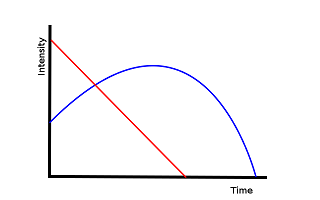
\includegraphics{time-intensity.png}
	\caption{intensity of sensory impression over time}
	\label{fig:time-intensity}
\end{figure}

\subsection{triangle test}
//todo


\section{Identification of the basic Flavor Types}
sweet \newline
4.5 g/l sugar \newline
bitter \newline
0,7 g/l caffeine \newline
sour \newline
0.4 g/l citric acid \newline
salty \newline
0.9 g/l sodium chloride \newline

\textcolor{red}{missing image}


\newpage
\section{Miscellaneous}
Before Sensorik you shall not:
\begin{itemize}
  \item smoke, because nicotine is a nerve poison and the flavor substances within
  the smoke distorts the overall gustatory perception
  \item eat chocolate
  \item use perfume
  \item forget to shower
\end{itemize}

\subsection{Advise for relishing Brewery Products}
crisp bread and water neutralizes the taste of previous samples. If there is no crisp bread in range
you can also use a simple wheat bun.
Also women are more sensitive to olfactory impulses. Furthermore they gustatory perceive
more intense in special ways including the bitterness. This leads to aversion of bitter beer
by most women. Rather useless is a sesame seed roll or something with sugar.
The flavor enhancing effect of sugar leads to misinterpretations.

Waiting 20 - 30 seconds helps to regain focus and get rid of this distracting predecessor.
At all cost overlay effects should be avoided.
Concentration is enormously important. It enhances sensibility and prevents
you from focusing on others.

\subsection{About the Lecturer}
Prof. Dr.-Ing. Frank-Jürgen Methner worked in research and development at Bitburger for 17 years.
He took part in the creation of "Koestritzer Schwarzbier" during the 90s.
At this time dark beer was rare. The only big brands were Koenig Ludwig dunkel and
Guinness.

Real beer needs a foam crown. A lack of tingling or foam can not be compensated,
not even with taste, temperature or visual appearance. Only true and desperate
thirst is an excuse to prevent the oncoming death with a sip of foam-free beer.


\end{document}
